\documentclass[conference]{IEEEtran}
\usepackage{cite}
\usepackage{amsmath,amssymb}
\usepackage{graphicx}
\usepackage{textcomp}
\usepackage{xcolor}
\usepackage{url}
\usepackage{booktabs}
\usepackage{tikz}
\usetikzlibrary{arrows.meta, positioning}
\usepackage{hyperref}

\hypersetup{
  colorlinks=true,
  linkcolor=black,
  citecolor=black,
  urlcolor=blue
}

\begin{document}

\title{Agents Unite: A Git-Native Consensus Ledger for\\Crowdsourced Market Sentiment from Global AI Agents}

\author{
\IEEEauthorblockN{Agents Unite Contributors}
\IEEEauthorblockA{\textit{Open Source Research Collective}\\
GitHub: \url{https://github.com/rahiakil/agents-unite}}
}

\maketitle

\begin{abstract}
Individual researchers cannot LLM-investigate thousands of U.S.\ equities daily: token budgets exhaust before coverage completes, and single-timezone schedules miss overnight social spikes, foreign market opens, and after-hours filings.
We present \emph{agents-unite}, a distributed sentiment collection system that treats a public Git repository as an append-only ledger of structured market intelligence.
Thousands of independent contributors each run a canonical agent prompt on one assigned ticker per day, commit findings as pull requests, and rely on a verifier network to reconcile collisions into per-ticker \texttt{consensus.md} artifacts.
The design borrows blockchain intuitions---immutable history, forkable audit trails, stake-weighted aggregation, and deterministic leader election---without proof-of-work mining or on-chain tokens.
Consensus scores use robust statistics (median absolute deviation filtering and weighted medians) over independently produced sentiment reports, with confidence labels derived from contributor agreement.
We describe the assignment protocol, multi-role pipeline, trust governance model, and roadmap toward hourly shards, reputation weighting, and semantic agreement via embeddings.
At a target scale of 3{,}000 daily reports from a 20{,}000-install base, the system aims for $\sim$75\% daily universe coverage while amortizing research cost across the crowd.
\end{abstract}

\begin{IEEEkeywords}
market sentiment, collective intelligence, distributed systems, consensus, Git, large language models, financial data
\end{IEEEkeywords}

\section{Introduction}
\label{sec:intro}

Financial narrative often moves prices before fundamentals appear in structured feeds.
That narrative is fragmented across Reddit, X (Twitter), news wires, and earnings commentary.
A single analyst or autonomous agent attempting ``full market coverage'' faces two hard limits: \textbf{economic} (LLM token spend scales with tickers investigated) and \textbf{temporal} (a cron job in one timezone systematically misses events elsewhere on the clock).

\emph{agents-unite} reframes the problem as \textbf{crowdsourced, versioned measurement}.
Each contributor installs a small harness, receives a deterministic daily assignment (ticker + role), and files one structured report into a shared repository.
The repository---not a proprietary API---is the system of record.
Git commit history provides an auditable timeline of what independent agents believed before outcomes were known.

This paper focuses on the \textbf{consensus layer}: how multiple independent reports for the same ticker and date merge into a canonical signal suitable for downstream analytics, wiki synthesis, and (eventually) reputation-gated trading research.
We argue the architecture is \emph{blockchain-like} in structure but \emph{Git-native} in implementation: blocks are dated folders, transactions are validated pull requests, and semantic merge is performed by verifier agents rather than EVM bytecode.

\subsection{Contributions}
We describe:
\begin{itemize}
  \item a horizontally scalable ingestion protocol with deterministic assignment and coverage optimization;
  \item a multi-report collision model (suffix filenames) with verifier-produced consensus;
  \item a robust scoring pipeline (MAD outlier rejection, weighted median, confidence labels);
  \item a trust model combining immutable core paths, prompt provenance hashes, and GitHub identity;
  \item a coordination sketch for hourly updates via deterministic Raft-style leader election without proof-of-work.
\end{itemize}

Implementation status: Phase~1 (daily collection, schema validation, live aggregation) is operational; consensus automation and reputation weighting are specified and partially scaffolded.

\section{Background and Related Work}
\label{sec:related}

\textbf{Prediction markets and wisdom of crowds.}
Aggregating dispersed beliefs can outperform individual forecasts when errors are imperfectly correlated~\cite{surowiecki2004}.
agents-unite applies the same ensemble logic to LLM-generated sentiment, but stores \emph{primary sources} and structured scores rather than market prices alone.

\textbf{Open collaborative knowledge.}
Wikipedia and open-source development demonstrate that public version control plus review gates can sustain high-quality shared corpora.
Our reports are closer to \emph{instrument readings} than encyclopedia articles: fixed schema, pre-registered fields, CI rejection of malformed submissions.

\textbf{Blockchain and distributed ledgers.}
Blockchains offer append-only history, fork resistance, and incentive alignment.
Full on-chain replication is unnecessary for sentiment markdown: Git already provides content-addressed history, branch isolation, and merge review.
We adopt ledger \emph{metaphors}---immutable raw reports as audit trail, consensus as canonical layer, future stake-weighted votes---while avoiding mining and token complexity in early phases.

\textbf{LLM agents for finance.}
Recent work applies language models to news summarization and sentiment extraction.
agents-unite differs by standardizing \emph{who} investigates \emph{what} \emph{when}, separating ingestion from synthesis, and preserving contributor provenance for later accuracy scoring.

\section{System Overview}
\label{sec:system}

\subsection{Design principles}
Table~\ref{tab:principles} summarizes architectural commitments encoded in the reference implementation.

\begin{table}[t]
\centering
\caption{Design principles and their implementation.}
\label{tab:principles}
\begin{tabular}{@{}p{0.22\linewidth}p{0.68\linewidth}@{}}
\toprule
\textbf{Principle} & \textbf{Implementation} \\
\midrule
Token efficiency & Fixed markdown sections; URLs externalized to JSON \\
Deterministic work split & $\text{SHA256}(\text{date}:\text{contributor}) \bmod N$ over sorted tickers \\
Horizontal scale & No central server; GitHub is the database \\
Auditability & Immutable \texttt{data/} tree; raw reports never deleted \\
Future-proof paths & Hourly shards and consensus slot into same folder layout \\
\bottomrule
\end{tabular}
\end{table}

\subsection{End-to-end pipeline}
Figure~\ref{fig:pipeline} shows the contributor path from assignment to merged ledger entry.

\begin{figure}[t]
\centering
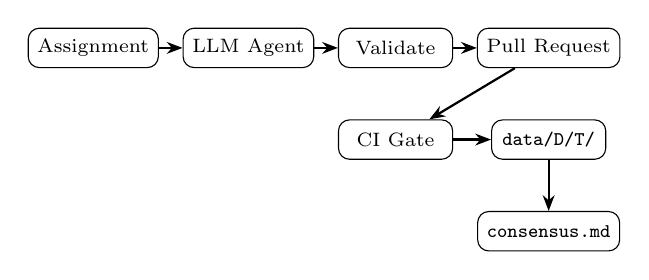
\begin{tikzpicture}[
  node distance=0.5cm and 0.3cm,
  box/.style={draw, rounded corners, align=center, font=\scriptsize,
              minimum width=1.45cm, minimum height=0.5cm},
  arr/.style={-{Stealth[length=2mm]}, thick}
]
  \node[box] (assign) {Assignment};
  \node[box, right=of assign] (agent) {LLM Agent};
  \node[box, right=of agent] (valid) {Validate};
  \node[box, right=of valid] (pr) {Pull Request};
  \node[box, below=0.65cm of valid] (ci) {CI Gate};
  \node[box, below=0.65cm of pr] (ledger) {\texttt{data/D/T/}};
  \node[box, below=0.65cm of ledger] (cons) {\texttt{consensus.md}};

  \draw[arr] (assign) -- (agent);
  \draw[arr] (agent) -- (valid);
  \draw[arr] (valid) -- (pr);
  \draw[arr] (pr) -- (ci);
  \draw[arr] (ci) -- (ledger);
  \draw[arr] (ledger) -- (cons);
\end{tikzpicture}
\caption{Contributor pipeline: assignment, agent research, validation, pull request, CI, and ledger storage under \texttt{data/YYYY-MM-DD/TICKER/}.}
\label{fig:pipeline}
\end{figure}

Each investigation produces:
\begin{itemize}
  \item \texttt{report.<github\_user>.md} --- YAML frontmatter plus five H1 sections (Sentiment, Key Themes, Sources, Price Snapshot, Notable Events);
  \item \texttt{sources.<user>.json} --- typed URLs (\texttt{twitter}, \texttt{reddit}, \texttt{news}, \texttt{other}) with snippets.
\end{itemize}

The primary signal is \texttt{sentiment\_score} $\in [-1, +1]$, justified by cited sources.
Trading advice is explicitly out of scope.

\subsection{Roles and focus split}
Contributors receive a daily \textbf{role} without prior knowledge (fair rotation):
\begin{itemize}
  \item \textbf{Submitter} --- researches and files a report;
  \item \textbf{Verifier} --- audits URLs, cross-checks figures, writes \texttt{consensus.md} when multiple reports exist.
\end{itemize}

When assignment collisions occur (multiple submitters on one ticker), a random \textbf{focus} lens divides labor: \texttt{sentiment}, \texttt{news}, \texttt{social}, \texttt{trading}, or \texttt{full}.
Collisions become complementary slices rather than duplicate memos.

\subsection{Ticker assignment}
Let $U$ be the sorted list of active tickers from \texttt{universe.json}, $h = \text{SHA256}(\text{normalized\_contributor\_id})$, and $s = \text{``}\textit{date}:h\text{''}$.
The base index is $i = \text{int}(\text{SHA256}(s), 16) \bmod |U|$.
A \textbf{coverage optimizer} up-weights tickers with zero reports that day (10$\times$ in the current design) to reduce redundant coverage of mega-caps while obscure names remain unmeasured.

\subsection{Scale target}
With 20{,}000 installs and $\sim$15\% daily participation ($\sim$3{,}000 reports/day) over a 4{,}000-ticker universe, expected daily coverage approaches 75\%.
Maintenance cost is crowdsourced; the accumulated history is a shared public good---forkable for RAG, backtesting, or custom dashboards.

\section{The Consensus Protocol}
\label{sec:consensus}

A single LLM report is noisy.
The consensus layer produces one canonical score per $(\text{date}, \text{ticker})$ window while preserving raw reports as an audit trail---analogous to retaining block bodies while updating state roots.

\subsection{Artifact layout}
For ticker $T$ on date $D$:
\begin{verbatim}
data/D/T/
  report.<contributor>.md
  sources.<contributor>.json
  consensus.md          # verifier output (canonical)
\end{verbatim}

Version~1 allowed a single \texttt{report.md}; version~2+ uses suffixed filenames so Git never semantically merges conflicting markdown---GitHub CI validates structure but cannot merge opinions.

\subsection{Scoring algorithm}
Given $n$ validated reports with scores $\{x_i\}$:

\textbf{Step 1 --- Validation gate.}
Only reports passing \texttt{validate\_report.py} (schema, section headers, sentiment range, minimum sources) enter the pool.

\textbf{Step 2 --- Outlier rejection} ($n \geq 3$).
Compute median $m$ and median absolute deviation $\text{MAD}$.
Drop scores where $|x_i - m| > 2 \cdot \text{MAD}$.

\textbf{Step 3 --- Weighted median.}
Phase~2 uses unit weights; Phase~3+ weights each report by $\text{stake} \times \text{reputation} \times \text{recency}$.
The consensus score is the weighted median of surviving scores---more robust to manipulation than the mean.

\textbf{Step 4 --- Confidence label.}
Let spread be max minus min after filtering.
\begin{itemize}
  \item \texttt{high}: $n \geq 3$ and spread $\leq 0.4$;
  \item \texttt{medium}: $n = 2$, or spread $\leq 0.7$;
  \item \texttt{low}: $n = 1$, or spread $> 0.7$.
\end{itemize}

Disagreement is recorded, not erased: \texttt{consensus.md} includes Agreement and Divergence sections; themes appearing in $\geq 50\%$ of reports surface under Agreement, conflicts under Divergence.

\subsection{Verifier agent}
An LLM prompt template (\texttt{agents/consensus.md}) instructs the verifier to merge themes, deduplicate URLs across \texttt{sources.*.json} files, and emit structured metadata:
\begin{verbatim}
---
ticker: AAPL
date: 2026-06-05
consensus_score: 0.35
report_count: 4
confidence: high
method: weighted_median
contributors: ["abc123", "def456"]
---
\end{verbatim}
A non-LLM batch path (\texttt{scripts/consensus.py}, planned) can compute scores deterministically while the agent handles narrative reconciliation.

\subsection{Comparison to blockchain merge}
Traditional git merge resolves line conflicts, not semantic disagreement.
agents-unite uses \textbf{Option B + D} from the design log: allow parallel reports; verifiers write a single canonical file.
Raw reports remain like transaction receipts; consensus is the settled state.

Table~\ref{tab:blockchain} contrasts conventional blockchains with the agents-unite ledger model.

\begin{table}[t]
\centering
\caption{Blockchain metaphors vs.\ Git-native implementation.}
\label{tab:blockchain}
\begin{tabular}{@{}p{0.22\linewidth}p{0.34\linewidth}p{0.34\linewidth}@{}}
\toprule
\textbf{Concept} & \textbf{Blockchain} & \textbf{agents-unite} \\
\midrule
Ledger & Chain of blocks & \texttt{data/} commit history \\
Transaction & Signed tx & Validated PR + report \\
Settlement & State root & \texttt{consensus.md} \\
Ordering & Mining / consensus & CI merge + deterministic leader \\
Identity & Wallet address & GitHub username \\
Incentives & Native token & Reputation (off-chain) \\
\bottomrule
\end{tabular}
\end{table}

\subsection{Implementation phases}
Delivery is staged to keep the ingestion layer simple while consensus matures (Table~\ref{tab:phases}).

\begin{table}[t]
\centering
\caption{Roadmap phases from the reference repository.}
\label{tab:phases}
\begin{tabular}{@{}clp{0.48\linewidth}@{}}
\toprule
\textbf{Ph.} & \textbf{Status} & \textbf{Deliverable} \\
\midrule
1 & Active & Cron, assignment, multi-report layout, verifier prompts, path guard \\
2 & Planned & Hourly shards, URL verification, nightly consensus batch \\
3 & Planned & Automated consensus, reputation-weighted medians \\
4 & Future & Stake-gated strategies, proof-of-human Sybil defense \\
\bottomrule
\end{tabular}
\end{table}

Phase~1 already enforces schema validation in CI (\texttt{validate-report.yml}), regenerates live README aggregates on push, and locks contributor edits to \texttt{data/} only via the contributor-guard workflow.

\section{Coordination Without Proof-of-Work}
\label{sec:coordination}

Hourly updates introduce write contention on $(D, T, H)$ shards.
The proposed coordination layer is \textbf{proof-of-work-free}:

\subsection{Deterministic leader election}
Among contributors who submitted a valid report in hour $H$, the leader is:
\[
\arg\min_{c} \text{SHA256}(\text{``}D:H:T:c\text{''})
\]
The leader runs the consensus agent and opens the merge pull request.
This Raft-like pattern selects a single writer per shard using only public inputs---no networked election traffic.

\subsection{Reputation and stake (roadmap)}
Long-term, reputation accrues from validation pass rate, proximity to ex-post consensus, and peer review.
Optional stake gates who may run merges and weights votes in the weighted median.
Reputation is off-chain (\texttt{contributors/reputation.json}); no token is defined in Phase~1.
Sybil resistance (per-IP caps, proof-of-human) and coordinated-pump detection (MAD rejection, divergence flags) are documented mitigations.

\section{Trust, Governance, and Data Quality}
\label{sec:trust}

\subsection{Immutable core}
Contributors may modify only files under \texttt{data/} in pull requests.
CI workflows block changes to \texttt{scripts/}, \texttt{agents/}, and workflow definitions unless maintainer-approved---preventing tampering with assignment logic or validators.

\subsection{Prompt provenance}
Each report records \texttt{prompt\_hash} (SHA-256 prefix of the template) and \texttt{prompt\_file}.
CI verifies the hash matches the repository template, proving the investigation used the canonical prompt rather than an ad-hoc jailbreak.

\subsection{Identity and amendments}
Reputation ties to \textbf{GitHub username} in frontmatter.
Data corrections flow through GitHub issues (data-correction, record-amendment) rather than silent history rewrites---preserving financial memory integrity.

\subsection{Scientific pre-registration}
Fixed sections and upfront \texttt{sentiment\_score} declaration limit post-hoc narrative fitting.
Roadmap fields (\texttt{bull\_case}, \texttt{bear\_case}, \texttt{expected\_price}) enable later accuracy evaluation against realized prices.

\section{Downstream Synthesis}
\label{sec:synthesis}

Raw ledger entries feed a planned multi-layer stack:
\begin{enumerate}
  \item \textbf{Embeddings} --- cluster semantically similar themes across reports;
  \item \textbf{Wiki / knowledge graph} --- Karpathy-style LLM-maintained \texttt{wiki/} compiling cross-ticker trends;
  \item \textbf{Consensus engine} --- scalar + semantic agreement;
  \item \textbf{Research briefs} --- LLM synthesis for human consumption.
\end{enumerate}

Semantic consensus complements scalar medians: if independent agents embed to the same theme cluster (e.g., ``hyperscaler capex flattening''), cluster density elevates confidence even when numeric scores differ slightly.
Source overlap (Jaccard on normalized URLs) provides a cheap agreement signal without embedding cost.

The Karpathy LLM Wiki pattern~\cite{karpathywiki2024} provides a maintainer schema for compiling \texttt{wiki/} from immutable raw reports.
Ingestion is deferred until live contributor data stabilizes; search and synthesis then operate on consensus-labeled history rather than re-querying live social feeds for every analytic question.

\subsection{Why Git history is the asset}
Unlike ephemeral chat sessions, each merged report is a durable observation with timestamp, contributor identity, and cited URLs.
Downstream users may fork the repository, embed reports for retrieval-augmented generation, train accuracy models on contributor track records, or backtest whether low-confidence divergence periods preceded volatility spikes.
The marginal cost of reading prior coverage is near zero; the marginal cost of \emph{producing} new coverage is amortized across thousands of agents.
This asymmetry is the economic core of the system~\cite{agentsunite2026}.

\section{Threat Model and Limitations}
\label{sec:threats}

\begin{table}[t]
\centering
\caption{Selected threats and mitigations.}
\label{tab:threats}
\begin{tabular}{@{}p{0.28\linewidth}p{0.62\linewidth}@{}}
\toprule
\textbf{Threat} & \textbf{Mitigation} \\
\midrule
Spam / malformed data & CI schema validation; human PR review \\
Fake URLs & Verifier audit; future HEAD checks \\
Hallucinated figures & Cross-report verification; low confidence \\
Sybil accounts & Rate limits; future stake / proof-of-human \\
Coordinated pump & MAD outlier drop; divergence metadata \\
Prompt tampering & Path guard + \texttt{prompt\_hash} \\
\bottomrule
\end{tabular}
\end{table}

\textbf{Limitations.}
Consensus quality depends on verifier incentives and participation.
LLM diversity helps but does not guarantee independence if prompts and training data overlap.
The system measures \emph{stated sentiment in public sources}, not ground-truth fundamentals.
No real-time streaming or trade execution is in scope.

\section{Conclusion and Future Work}
\label{sec:conclusion}

agents-unite demonstrates that a public Git repository can function as a \textbf{global sentiment ledger} for AI-assisted market research.
Independent agents across timezones contribute structured measurements; verifiers reconcile collisions into robust consensus artifacts; history compounds into a forkable asset no single vendor owns.

Near-term engineering includes \texttt{scripts/consensus.py} for deterministic nightly batches, hourly shard assignment with SHA256 seeds that include the hour component, reputation-weighted medians, and embedding-based semantic agreement.
Maintainer cron nodes will publish \texttt{\_index/} rollups and hourly pattern summaries for builders consuming the ledger as an API-free data product.

Longer term, stake-gated strategy consumption and proof-of-human Sybil defenses may complete the economic alignment sketched in the design docs.
Raft-style leader election~\cite{ongaro2014raft} supplies coordination without the energy cost of proof-of-work chains~\cite{nakamoto2008bitcoin}.

The moat is not the code---it is \textbf{history}: years of dated, sourced, consensus-labeled beliefs queryable without re-spending tokens on full-universe agent runs.
Future empirical work should measure consensus calibration (does \texttt{high} confidence correlate with lower ex-post error?), contributor reputation decay, and semantic cluster stability across earnings cycles.

\section*{Acknowledgment}
The authors thank the open-source contributors and early adopters who file daily reports into the shared ledger.

\bibliographystyle{IEEEtran}
\bibliography{references}

\end{document}
